\documentclass[mathserif]{beamer}

%%%%%%%%%%%%%%%%%%%%%%%%%%%%%%%%%%%%%%%%%%%%%%%%%%%%%%%%%%%%%%%%%%%%%%%%%%%%%%%%
%% Beamer
%%%%%%%%%%%%%%%%%%%%%%%%%%%%%%%%%%%%%%%%%%%%%%%%%%%%%%%%%%%%%%%%%%%%%%%%%%%%%%%%

\mode<presentation>
{
 \usetheme{Madrid}
 \setbeamercovered{transparent}
}


%%%%%%%%%%%%%%%%%%%%%%%%%%%%%%%%%%%%%%%%%%%%%%%%%%%%%%%%%%%%%%%%%%%%%%%%%%%%%%%%
%% Packages
%%%%%%%%%%%%%%%%%%%%%%%%%%%%%%%%%%%%%%%%%%%%%%%%%%%%%%%%%%%%%%%%%%%%%%%%%%%%%%%%

\usepackage{hyperref}
\usepackage{amsfonts}
\usepackage[english]{babel}
\usepackage{times}
\usepackage[T1]{fontenc}
\usepackage{xspace}
\usepackage{graphicx}
\usepackage[utf8]{inputenc}
\usepackage[normalem]{ulem}

\usepackage{tikz}
\usetikzlibrary{positioning}    %needed for e.g. ``right=5em of ..''
\usetikzlibrary{calc}
\usepackage{url}


%%%%%%%%%%%%%%%%%%%%%%%%%%%%%%%%%%%%%%%%%%%%%%%%%%%%%%%%%%%%%%%%%%%%%%%%%%%%%%%%
%%% Title
%%%%%%%%%%%%%%%%%%%%%%%%%%%%%%%%%%%%%%%%%%%%%%%%%%%%%%%%%%%%%%%%%%%%%%%%%%%%%%%%


\title[]{Interactive Control of Diverse Complex Characters with Neural Network}
\author[]{Jules Kozolinsky}
\date[]{23 janvier 2017}


%%%%%%%%%%%%%%%%%%%%%%%%%%%%%%%%%%%%%%%%%%%%%%%%%%%%%%%%%%%%%%
%%%%%%%%%%%%%%%%%%%%%%%%%%%%%%%%%%%%%%%%%%%%%%%%%%%%%%%%%%%%%%
%%%%%%%%%%%%%%%%%%%%%%%%%%%%%%%%%%%%%%%%%%%%%%%%%%%%%%%%%%%%%%



\begin{document}

%--------------------------------------------------------------

\begin{frame}
  \begin{center}

    \begin{minipage}{.9\textwidth}
      \begin{block}{}
	\begin{center}
	  \Large Interactive Control of Diverse Complex Characters with Neural Network
	\end{center}
      \end{block}
    \end{minipage}

  \vspace*{20pt}
  Igor Mordatch, Kendall Lowrey, Galen Andrew, \\
  Zoran Popovic, Emanuel V. Todorov



 \vspace*{10pt}
  {\small University of Washington}

  \vspace*{2cm}
Paper presentation for robotics class \\
Jules Kozolinsky\\
23 January 2017

  \end{center}
\end{frame}



%------------------------------------------------------------------------------
%---------------------------------------------------------------------- SLIDE -


%% \begin{frame}%<beamer>
%%     \frametitle{Outline}
%%     \tableofcontents
%%   \end{frame}



%------------------------------------------------------------------------------
%---------------------------------------------------------------------- SLIDE -



%% \AtBeginSection[]{%
%%   \begin{frame}%<beamer>
%%     \frametitle{Outline}
%%     \tableofcontents[sectionstyle=show/shaded,subsectionstyle=show/show/hide]
%%   \end{frame}
%% }



%------------------------------------------------------------------------------
\section{Introduction}
%---------------------------------------------------------------------- SLIDE -

\begin{frame}
  \frametitle{{Context}}
  
\begin{block}{Context of the article}
\begin{itemize}
\item Title : \textit{Interactive Control of Diverse Complex Characters with Neural Network}
\item Authors : Igor Mordatch, Kendall Lowrey, Galen Andrew, Zoran Popovic, Emanuel V. Todorov
\item[] from the Department of Computer Science, University of Washington
\item published in NIPS 2015 (Neural Information Processing Systems)
\end{itemize}
\end{block}

\end{frame}

%------------------------------------------------------------------------------
%---------------------------------------------------------------------- SLIDE -

\begin{frame}
  \frametitle{{Goal of the article}}
  
  Interactive real-time controllers (generating complex, stable and realistic movements) have many potential applications.
  
\begin{block}{State of the art of controllers designing}
\begin{itemize}
\item time-consuming
\item largely manual 
\item relying on motion capture datasets
\end{itemize}
\end{block}

\pause

\begin{block}{Goal}
Automate this process, \textit{i.e.} find a policy 
\begin{itemize}
\item universal methods applicable to arbitrary behaviors or body morphologies
\item online changes in task objectives
\item perturbations due to noise and modelling errors
\end{itemize}
\end{block}


\end{frame}

%------------------------------------------------------------------------------
%---------------------------------------------------------------------- SLIDE -

\begin{frame}
  \frametitle{{How?}}
  \begin{block}{Trajectory optimization}
  \begin{itemize}
  \item Contact-Invariant-Optimization \cite{mordatch2012discovery}
  \item Offline method to find a optimal trajectory
  \end{itemize}
  
  \end{block}
  \begin{block}{Deep learning}
  \begin{itemize}
  \item supervised learning using neural network 
  \item normally used in speech-recognition or computer vision
  \end{itemize}
  \end{block}
  
  \vspace{1cm}
 \textbf{Method :} neural network learn from the optimizer and generate similar behaviour online 
  

\end{frame}

%------------------------------------------------------------------------------
%---------------------------------------------------------------------- SLIDE -

\AtBeginSection[]{%
  \begin{frame}%<beamer>
    \frametitle{Outline}
    \tableofcontents[sectionstyle=show/shaded,subsectionstyle=show/show/hide]
  \end{frame}
}

%------------------------------------------------------------------------------
\section{Overview}
\subsection{Problem}
%---------------------------------------------------------------------- SLIDE -

\begin{frame}
  \frametitle{{Definitions}}
  \begin{block}{State of character and trajectory}
  \begin{itemize}
  \item State of character : $(q~f~r)$ 
  \begin{itemize}
  \item[] $q$ physical pose (position, orientation, joint angles)
  \item[] $f$ contact forces 
  \item[] $r$ recurrent memory
  \end{itemize}
  \item Trajectory of length $T$ : $(q^0~f^0~r^0~...~q^T~f^T~r^T)$ 
  \end{itemize}
  \end{block}
\end{frame}

%------------------------------------------------------------------------------
%---------------------------------------------------------------------- SLIDE -

\begin{frame}
  \frametitle{{Definitions}}
  \begin{block}{Neural network policy }
  \begin{align*}
  \pi_{\theta} : s \mapsto a
  \end{align*}
  where 
  \begin{itemize}
  \item $\theta$ neural network weight
  \item $s^t(X) = (q^t~r^t~\dot{q}^{t-1}~f^{t-1})$  sensory state a time $t$ of trajectory $X$
  \item $a^t(X) = (\dot{q}^{t}~\dot{r}^{t}~f^{t})$ optimal action a time $t$ of trajectory $X$
  \item[] ($\dot{x}^t = x^{t+1}-x^t$)
  \end{itemize}
  \end{block}

\vspace{20pt}

\textbf{Note :} The neural network learns both optimal control and model of dynamics  
  
\end{frame}
%------------------------------------------------------------------------------
%---------------------------------------------------------------------- SLIDE -

\begin{frame}
  \frametitle{{Problem}}
  \begin{block}{Offline procedure}
  \begin{align}
  \min_{\theta,X^1,...,X^N} \sum\limits_{i=1}^{N} C_{i}(X^{i}) \hspace{15pt}\text{ \small subject to } \hspace{5pt} \forall i,t : a^{t}(X^{i}) = \pi_{\theta}(s^{t}(X^{i}))
  \end{align}
  where 
  \begin{itemize}
  \item $\theta$ policy parameters ($\pi_{\theta} : s \mapsto a$) 
  \item $X^{i}$ trajectory of task $i$ (different initial conditions)
  \end{itemize}
  \end{block}

\vspace{20pt}

\textbf{Note :} Then optimized policy parameter $\theta^{*}$ is used to execute policy in real-time

\end{frame}


%------------------------------------------------------------------------------
\subsection{Stochastic Policy and Sensory Inputs}
%---------------------------------------------------------------------- SLIDE -

\begin{frame}
  \frametitle{{Noise into the sensory inputs}}
  \begin{block}{Why add noise?}
  \begin{itemize}
  \item Produce more robust movement stategies \cite{huh2009real} \cite{wang2010optimizing}
  \item Reduce overfitting \cite{hinton2012improving}
  \item Stabilize behaviour of neural network \cite{hoerzer2014emergence}
  \end{itemize}
  Main reason :  Learning policy does not diverge at execution time
  \end{block}
\end{frame}


%------------------------------------------------------------------------------
%---------------------------------------------------------------------- SLIDE -

\begin{frame}
  \frametitle{{Noise into the sensory inputs}}
   \begin{block}{How to add noise?}
  Add gaussian noise into inputs $s$ given to the neural network : 
  \begin{align*}
  \pi_{\theta}(s + \varepsilon) = a + a_{s}\varepsilon 
  \end{align*}
  where 
  \begin{itemize}
  \item $\varepsilon \sim \mathcal{N}(0,\sigma_{\varepsilon}^{2}I)$ \hspace{5mm} ($\sigma_{\varepsilon}^{2} \simeq 10^{-2}$)
  \item $a_s$ gradient in first order expansion : matrix of optimal feedback (Section 3 for analytic calculation)
  \end{itemize}
  \end{block}
  
  \vspace{20pt}

\textbf{Note :} Policy automatically corrects small deviations from the optimal trajectory
\end{frame}


%------------------------------------------------------------------------------
\subsection{Algorithm}
%---------------------------------------------------------------------- SLIDE -

\begin{frame}
  \frametitle{{Algorithm}}
  \begin{block}{Optimization under constraints}
  Problem $(1)$ non-convex : we replace the hard equality constraint
  \begin{align*}
  \min_{\theta,X^1,...,X^N} \sum\limits_{i=1}^{N} C_{i}(X^{i}) + \sum\limits_{i,t} R(s^{t}(X^{i}),a^{t}(X^{i}),\theta,\varepsilon^{i,t})\\ \text{\footnotesize with } \hspace{5pt}
  R(s,a,\theta,\epsilon) = \frac{\alpha}{2}||(a+a_s\varepsilon) - \pi_{\theta}(s+\epsilon)||^2
  \end{align*}
  where 
  \begin{itemize}
  \item $\theta$ policy parameters ($\pi_{\theta} : s \mapsto a$) 
  \item $X^{i}$ trajectory of task $i$
  \item $\alpha$ weight on quadratic penalty ($\alpha \simeq 10$)
  \end{itemize}
  \end{block}

\end{frame}


%------------------------------------------------------------------------------
%---------------------------------------------------------------------- SLIDE -

\begin{frame}
  \frametitle{{Algorithm}}
  \begin{block}{Algorithm}
\begin{enumerate}
\item Sample noise $\varepsilon^{i,t}$
\item Optimize $N$ trajectories : 
\begin{align*}
\forall i, \hspace{3pt} \bar{X}^{i} = \text{argmin}_{X} ~C_{i}(X) + \sum_{t} R(s^t(X),a^t(X),\bar{\theta},\bar{\varepsilon}^{i,t}) + \frac{\eta}{2}||X-\bar{X}^{i}||^2
\end{align*}
\item Train neural network : 
\begin{align*}
\bar{\theta} = \text{argmin}_{\theta} ~\sum_{i,t} R(s^t(\bar{X}_i),a^t(\bar{X}_i),\theta,\bar{\varepsilon}^{i,t}) + \frac{\eta}{2}||\theta-\bar{\theta}||^2
\end{align*}
\item Repeat
%TODO until ? 
\end{enumerate}
  \end{block}
{\small ($\eta \simeq 10^{-2}$)}
\end{frame}


%------------------------------------------------------------------------------
%---------------------------------------------------------------------- SLIDE -

\AtBeginSection[]{%
  \begin{frame}%<beamer>
    \frametitle{Outline}
    \tableofcontents[sectionstyle=show/shaded,subsectionstyle=show/show/hide]
  \end{frame}
}

%------------------------------------------------------------------------------
\section{Trajectory Optimization}
\subsection{Physical realism}
%---------------------------------------------------------------------- SLIDE -

\begin{frame}
  \frametitle{{Trajectory Optimization}}
  \begin{block}{Step 2 of the algorithm}
  \begin{align*}
  \bar{X} = \text{argmin}_{X} ~C_{i}(X) + \sum_{t} R(s^t(X),a^t(X),\bar{\theta},\bar{\varepsilon}^{i,t}) + \frac{\eta}{2}||X-\bar{X}||^2
  \end{align*}
  
  \vspace{15pt}
  
    Find trajectories that start with partiular inital conditions and execute the task, while satisfying physical realism of character's motion.
  \end{block}

\end{frame}


%------------------------------------------------------------------------------
%---------------------------------------------------------------------- SLIDE -

\begin{frame}
  \frametitle{{Trajectory Optimization}}
  \begin{block}{Physical realism}
  \begin{align*}
H(q)\ddot{q} + \hat{C}(q,\dot{q}) = \tau + J(q,\dot{q})^{\top}f, \hspace{15pt}
 d(q) \geq 0,  \hspace{10pt}
 d(q)^{\top}f = 0,  \hspace{10pt}
 f \in K(q) 
  \end{align*}
  where 
  \begin{itemize}
  \item $f$ contact forces acting on all end-effectors
  \item $\tau$ inverse of the dynamics
  \item $H$ the inertia matrix
  \item $\hat{C}$ the matrix of Coriolis and centrifugal terms
  \item $J$ Jacobian matrix 
  \item $d(q)$ distance of the contact to the ground 
  \item $K(q)$ contact friction cone
  \end{itemize}
  \end{block}
	
	These constraints and initial conditions are implemented as soft constraints and included in $C(X)$	
	
\end{frame}


%------------------------------------------------------------------------------
\subsection{Optimal trajectory}
%---------------------------------------------------------------------- SLIDE -

\begin{frame}
  \frametitle{{Optimal trajectory}}
  \begin{block}{Total cost}
  \begin{align*}
  C(X) = \sum\limits_{t}c^t(\phi^t(X))
  \end{align*}
  where
  \begin{itemize}
  \item $\phi^t(X)$ extracts features from trajectory
  \item $c(\phi)$ cost over these features
\end{itemize} 
  \end{block}
  
  
  \begin{block}{Optimization problem}
  For simplicity, objectives folded into $C$ : 
  \begin{align*}
  X^* = \text{argmin}_{X} C(X)
  \end{align*}
  \end{block}
  
\end{frame}


%------------------------------------------------------------------------------
%---------------------------------------------------------------------- SLIDE -

\begin{frame}
  \frametitle{{Newton's method}}
  \begin{block}{Gaussian-Newton Hessian approximation}
  \begin{align*}
  \nabla_{X}C(X) &= \sum\limits_{t}c_{\phi}^t\phi^t_{X} \\
  D^2_{X}C(X) &= \sum\limits_{t}(\phi^t_{X})^{\top}c_{\phi\phi}^t\phi^t_{X} + c_{\phi}^t\phi^{t}_{XX} \approx \sum\limits_{t}(\phi^t_{X})^{\top}c_{\phi\phi}^t\phi^t_{X}
  \end{align*}
  where
  \begin{itemize}
  \item $c(\phi)$ cost functions (gradient and hessian analytically calculable)
  \item $\phi_{X}^t$ calculated by finite differencing
\end{itemize} 
  \end{block}
  
   \begin{block}{Newton's method}
  \[
  X^{*} = X^{*} - D^2_{X}C(X)^{-1}\nabla_{X}C(X) 
  \]
  \textbf{Note :} Not run to convergence, only between $1$ and $10$ iterations
  \end{block}

\end{frame}


%------------------------------------------------------------------------------
\subsection{Optimal feedback gains}
%---------------------------------------------------------------------- SLIDE -

\begin{frame}
  \frametitle{{Optimal feedback gains}}
   \begin{block}{How to add noise? (Reminder)}
  Add gaussian noise into inputs $s$ given to the neural network : 
  \begin{align*}
  \pi_{\theta}(s + \varepsilon) = a + a_{s}\varepsilon 
  \end{align*}
  where 
  \begin{itemize}
  \item $\varepsilon \sim \mathcal{N}(0,\sigma_{\varepsilon}^{2}I)$ \hspace{5mm} ($\sigma_{\varepsilon}^{2} \simeq 10^{-2}$)
  \item $a_s$ gradient in first order expansion : matrix of optimal feedback
  \end{itemize}
  \end{block}
  
  \begin{block}{Perturbation of optimal trajectory}
  Let $\tilde{X}$ be the perturbation of optimal trajectory $X$ such that $s(\tilde{X}) = \bar{s} $. \\
  Then 
  \[
  a_{\bar{s}} = a_{X}\tilde{X}_{\bar{s}}
  \]
  \end{block}
  
  \end{frame}


%------------------------------------------------------------------------------
%---------------------------------------------------------------------- SLIDE -

\begin{frame}
	\frametitle{{Optimal feedback gains $a_{\bar{s}}$}}
	\begin{block}{Calculating $a_{X}$}
	$a$, $s$ and $\phi$ are functions that extract features overs $X$. \\
	So $s_X$ and $a_X$ are subsets of $\phi_X$. 
	\end{block}
	
  \begin{block}{Calculating $\tilde{X}_{\bar{s}}$}
  We have (with $\lambda \simeq 10^2$),
  \[
  \tilde{X}(\bar{s}) = \text{argmin}_{X^{*}} \big{(}C(X^{*}) + \frac{\lambda}{2}||s(X^{*}) - \bar{s}||^{2}\big{)}
  \]
    Then,
    \[
  \tilde{X}(\bar{s}) = X - (C_{XX} + \lambda s_{X}^{\top}s_{X})^{-1}(C_{X} + \lambda s_{X}^{\top}(s(X) - \bar{s})
  \]
  And, 
  \[
  \tilde{X}_{\bar{s}} = \lambda(C_{XX} + \lambda s_{X}^{\top}s_{X})^{-1}s_{X}^{\top}
  \]
  \end{block}
\end{frame}


%------------------------------------------------------------------------------
%---------------------------------------------------------------------- SLIDE -

\AtBeginSection[]{%
  \begin{frame}%<beamer>
    \frametitle{Outline}
    \tableofcontents[sectionstyle=show/shaded,subsectionstyle=show/show/hide]
  \end{frame}
}

%------------------------------------------------------------------------------
\section{Neural Network Training}
%---------------------------------------------------------------------- SLIDE -

\begin{frame}
  \frametitle{{Neural network training}}
  \begin{block}{Step 3 of the algorithm}
	\begin{align*}
\bar{\theta} = \text{argmin}_{\theta} ~\sum_{i,t} R(s^t(\bar{X}_i),a^t(\bar{X}_i),\theta,\bar{\varepsilon}^{i,t}) + \frac{\eta}{2}||\theta-\bar{\theta}||^2
	\end{align*}  
	with 
	\[
	 R(s,a,\theta,\epsilon) = \frac{\alpha}{2}||(a+a_s\varepsilon) - \pi_{\theta}(s+\epsilon)||^2
	 \]
  \end{block}
  
  \begin{block}{Neural network policy regression}
  \textbf{Training data : } $(s + \varepsilon, a + a_{s}\varepsilon)^{i,t}$ \\
  \vspace{10pt}
  \textbf{Output function : }  $\theta^{*}$ weight of neural network used in policy $\pi_{\theta^{*}} : s \mapsto a$
  
  \end{block}
\end{frame}


%------------------------------------------------------------------------------
%---------------------------------------------------------------------- SLIDE -

\begin{frame}
  \frametitle{{Neural network training}}
  \begin{block}{A difficult problem}
\begin{itemize}
\item data set harder to obtain (// computer vision)
\item regression (real valued outputs) $\not=$ classification (categorical outputs)
\item no i.i.d. values 
\end{itemize}
  \end{block}

\end{frame}


%------------------------------------------------------------------------------
%---------------------------------------------------------------------- SLIDE -

\begin{frame}
  \frametitle{{Neural network training}}
  \begin{block}{Parameters of the neural network}
\begin{itemize}
\item hidden layer activation function $\sigma = tanh$
\item 3 hidden layers with 250 hidden units in each layer
\item $\gamma \sim \mathcal{N}(0,\sigma_{\gamma}^{2}I)$ noise at each layer during training ($\sigma_{\gamma} \simeq 10^{-2}$)
\end{itemize}
  \end{block}
  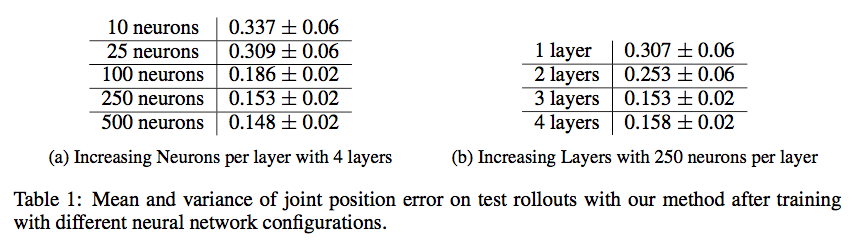
\includegraphics[scale=0.4]{nn}\\
  
\textbf{Note :} Not run to convergence
\end{frame}


%------------------------------------------------------------------------------
%---------------------------------------------------------------------- SLIDE -

\AtBeginSection[]{%
  \begin{frame}%<beamer>
    \frametitle{Outline}
    \tableofcontents[sectionstyle=show/shaded,subsectionstyle=show/show/hide]
  \end{frame}
}

%------------------------------------------------------------------------------
\section{Policy execution}
%---------------------------------------------------------------------- SLIDE -

\begin{frame}
  \frametitle{{Policy execution}}
  \begin{block}{Real-time execution}
  We found policy parameters $\theta^{*}$ offline. \\
  Let $x^0$ be the initial state. Then desired action : $a^{des} = \pi_{\theta^{*}}(s(x^0))$.
  So, 
  \[
  x^{1} = \text{argmin}_{x} ||\dot{q} - \dot{q}^{des}||^2 + ||\dot{r} - \dot{r}^{des}||^2 + ||f - f^{des}||^2 \hspace{3pt} \text{\small subject to dynamics}
  \]
  (same trajectory optimization problem with horizon $T=1$)
  \end{block}
 
\end{frame}


%------------------------------------------------------------------------------
%---------------------------------------------------------------------- SLIDE -

\AtBeginSection[]{%
  \begin{frame}%<beamer>
    \frametitle{Outline}
    \tableofcontents[sectionstyle=show/shaded,subsectionstyle=show/show/hide]
  \end{frame}
}

%------------------------------------------------------------------------------
\section{Results}
%---------------------------------------------------------------------- SLIDE -

\begin{frame}
  \frametitle{{Results}}
  \begin{block}{Set-up}
  \begin{itemize}
 	\item $\Delta t = 50$ ms
 	\item takes about $2.5$ hours
 	\item MuJoCo physics simulator 
  \end{itemize}
  \end{block}
  
  \begin{block}{Experiments}
  \begin{itemize}
 	\item swimming
 	\item flying
 	\item biped walk
 	\item quadruped walk
  \end{itemize}
 Video : \url{https://www.youtube.com/watch?v=IxrnT0JOs4o}
  \end{block}

\end{frame}


%------------------------------------------------------------------------------
%---------------------------------------------------------------------- SLIDE -

\begin{frame}
 \begin{center}
 \begin{Huge}
Conclusion and future work
\end{Huge}
 \end{center}

\end{frame}


%------------------------------------------------------------------------------
%---------------------------------------------------------------------- END ---


\bibliographystyle{plain}
\bibliography{biblio}
\end{document}
